\chapter{Решење проблема применом алгоритма моделовања тема }

Проналажење правог одговора на постављено питање може бити изузетно сложен проблем чак и за човека. Оно што је суштински важно за препознавање ваљаног одговора је разумевање \textbf{суштине} односно смисла питања. За разлику од машина, човек на основу знања, уме да наслути тај смисао а самим тим и да препозна адекватан одговор. Међутим, уколико би се пред човека ставило питање из области о којој он нема никаквог знања ( не разуме значење речи) или је на језику који не разуме, врло је вероватно да би препознавање правог одговора било јако непоуздано. 
Са друге стране, немогуће је не запитати се шта заправо представља прави одговор на постављено питање. Данас је можда лакше него икада поставити питање и у кратком времену добити велики број одговора од различитих корисника. Учесници конверзације не морају нужно бити стручњаци из области које се тиче питања. Исто тако, велики број одговора, иако су наизглед адекватни, наилазе на осуду стручне популације. Дакле, потребно је извесно време, у коме долазо до комуникације међу различитим корисницима ( давање оцена се може сматрати комуникацијим) да би се \textbf{закључило} шта је прави одговор. 
Сајтови који су служили као извор података су управо описаног карактера. Дакле, одговори на поствањено питање се оцењују од стране заинтересованих корисника и након неког времена са великом прецизношћу се може рећи који је адекватан одговор на постављено питање. Према томе, подаци који су овде разматрани јако су зависно од :

\begin{itemize}
\item атрактивности теме којом се баве - што је тема популарнија то ће већи број корисника бити укључен у давање и оцењивање одговора. Самим тим, може се сматрати да атрактивније теме имају поузданије одговоре
\item природе питања - на нека питања се може одговорити врло кратко - (на пример где се ПМФ налази у Крагујевцу ) док друга питања захтевају опширне одговоре (нпр. детаљан опис историје Крагујевца или препричано књижевно дело)
\end{itemize}

У правом одговору не морају нужно да се нађу речи из питања. Исто тако, не мора постојати законитост између дужине питања и одговора. Према томе, не постоји \textbf{алгоритам} којим се може закључити који је адекватан одговор а да се при томе не укљичи додатно експертско знање. 

Основна идеја овог рада је испитивање да ли се и у којој мери вештачно знање које се добија применом алгоритма моделовања тема може употребити за селектовање правог одговора без убацивања додатног експертског знања.


\section{Опис решења}

Идеја решења је изградња \textbf{модела тема} над свим одговорима чиме би се добио истрениран модел који поседује знање о том скупу докумената. Под знањем се подразумева расподела тема над документима као и расподела речи унутар тема. Основна предпоставка је да се при постављању питања то знање може употребити како би се селектовао тачан одговор. Даље сe претпоставља да су  питање и одговор  највероватније из истих области ( једна или више ) односно да говоре о истим темама. Овде је важно напоменути да теримн \textbf{област} или \textbf{тема} више није упоредив са човековим схватањем тема или области. Обзорим да је број тема који се у истраживању користио јако велики - од 100 до 2000 - и да тема није ништа друго до скуп речи као и да у систем није укључено никакво додатно експретско знање, ово напомена је сасвим очигледна.

Селектовање правог одговора вршено је мерењем \textbf{сличности} између постављеног питања и свих одговора. Онај одговор који је \textbf{најсличнији} постављеном питању, одабира се као тачан одговор на постављено питање. Обзиром да је познато који одговор припада ком питању, рад програма је једноставно проверити и измерити.

За мерење сличности питања и одговора коришћено је неколико метода које се разликују  по прецизности, брзини рада и меморијским захтевима. 


Идејни ток решења може се представити  дијаграмом као на слици 4.1:

\begin{figure}[H]
    \centering
   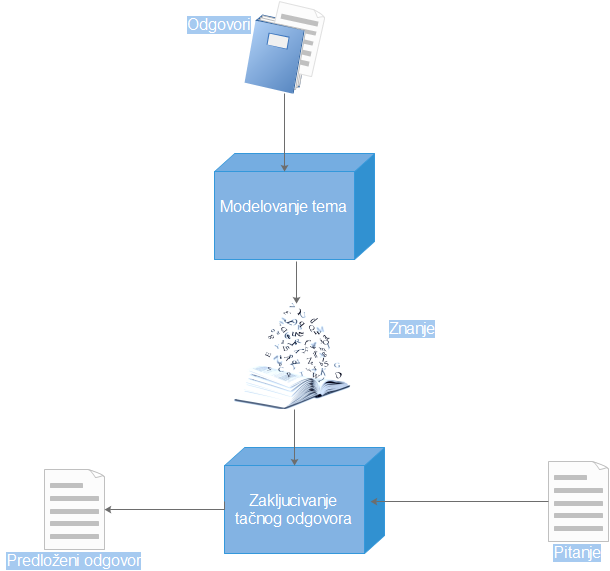
\includegraphics[scale=0.9]{./Slike/slika37.png} 
	\caption{Ток решења}
	\label{fig:slika1}
\end{figure}


\section{Мерење сличности}

Мерење сличности је од суштинске важности за одабирање одговора на поствањено питање. Она утиче на прецизност решења, брзину извршавања, меморијске захтеве итд. 



\subsection{Косинусна сличност}

Један од излаза алгоритама тема је и расподела тема по документима.Такође, за сваки нови документ, могуће је предвидети расподелу по темама. Дакле, пошто се вектор расподела по темама увек може направити, корисно их је искористити као меру сличности два документа.

Вектор расподеле по темама, дужине n може се замислити  као права у n-димензионаланом простору. Дакле, вектор питања и вектор одговора могу се замислити као две праве у n-димензионаланом. Што су те две праве "`ближе"' једна другој, односно што је угао између њих ближи 0, то су питање и одговор сличнији. 
Пошто се ради о расподелама, максимална вредност коју може да узме нека координата овако дефинисаног вектора је 1, док ј еминимална вредност 0, што значи да се обе праве налазе у првом квадранту. Дакле, максимални угао који два вектора могу да граде је 90 степени и , у смислу косинуссне мере, означава да су документи потпуно различити.
Близина праве питања и праве одговора означава сличну расподелу по темама. Ако се узме у обзор полазна претпоставка да питање и одговор "`говоре о"' истим темама, постаје јасно због чега се угао између ових правих може узети за меру сличности два документа.

Ради илустрације, следи један прилично упрошћен и нереалан пример. 
Нека је скуп свих могућих речи састављен од три речи : \textit{reč1,reč2,reč3} и нека су дате три реченице састављене од поменутих речи : \textit{rečenica1, rečenica2,rečenica3}. 
Дате реченице могу се графички представити као праве ( Слика)

\begin{figure}[H]
    \centering
   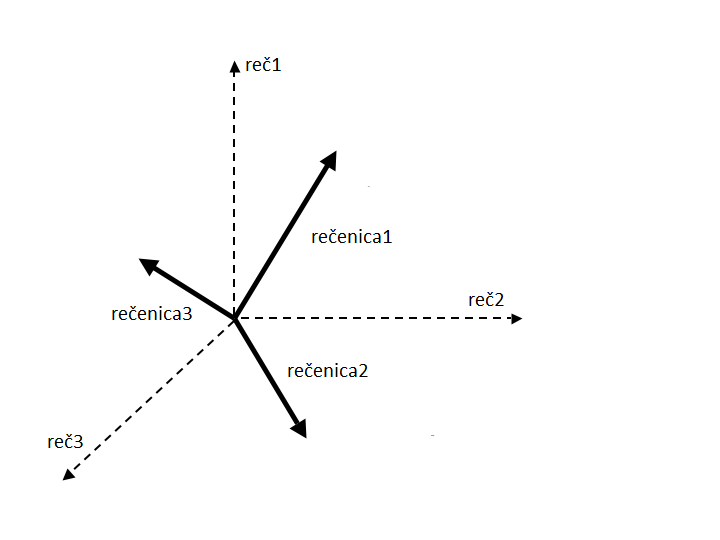
\includegraphics[scale=0.3]{./Slike/kosinusna.png} 
	\caption{Зависност просечне позиције од броја тема и броја итерација}
	\label{fig:slika1}
\end{figure}

Угао између сваке две праве представља меру сличности реченица.

Уместо мерења угла између два вектора, практичније је мерити косинус тог угла. 
Косинус угла који заклапају два вектора може се одредити следећом формулом :


$$ cos\theta = \frac{\overrightarrow{a}\cdot \overrightarrow{b}}{\Vert\overrightarrow{a}\Vert\overrightarrow{b}\Vert} $$




